\setlength{\tabcolsep}{0.1cm}
\begin{figure}
\begin{tabular}{c c c }
     Split1 & Split2 & Split3 
    \\
    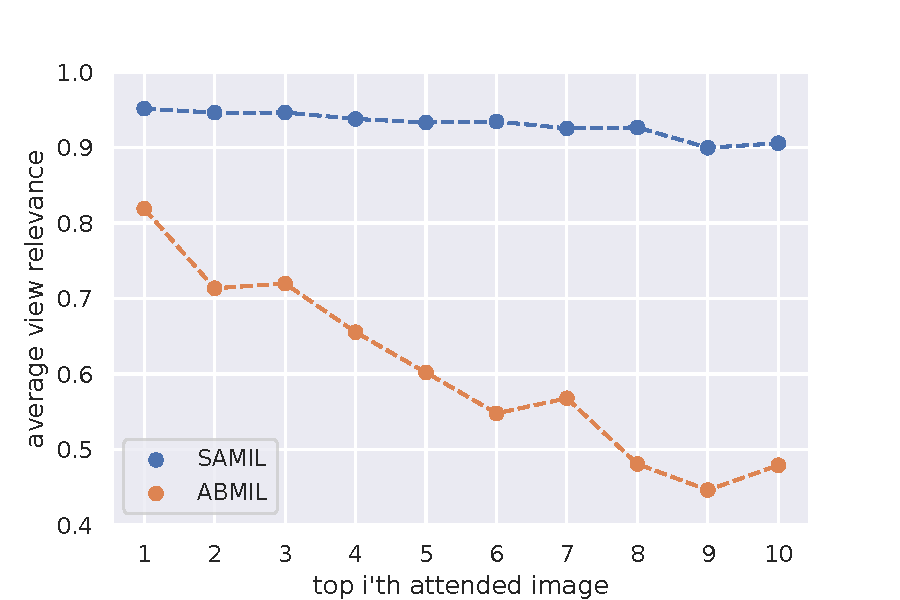
\includegraphics[width=0.32\textwidth]{figures/Attention_View_Alignment/data_seed0.pdf}
    &
    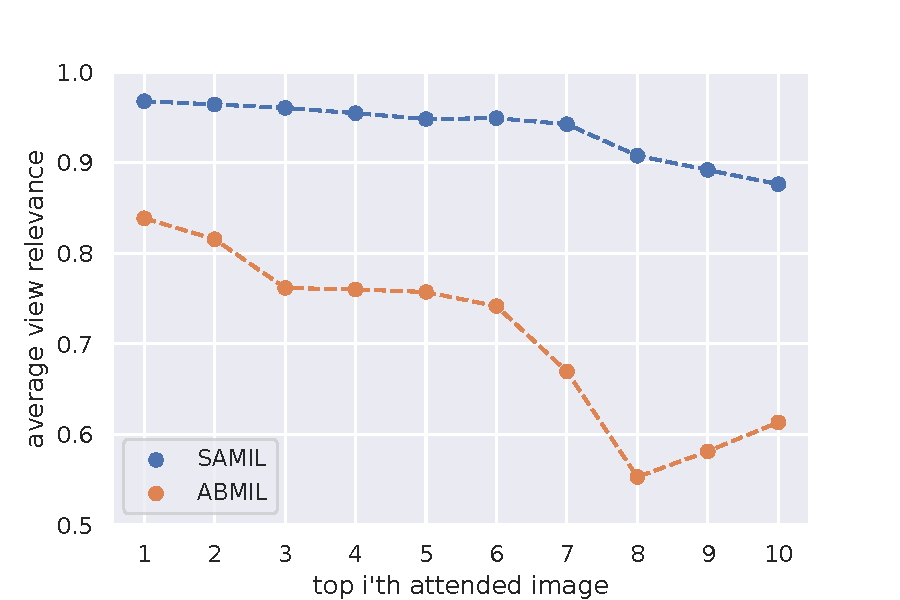
\includegraphics[width=0.32\textwidth]{figures/Attention_View_Alignment/data_seed1.pdf}
    &
    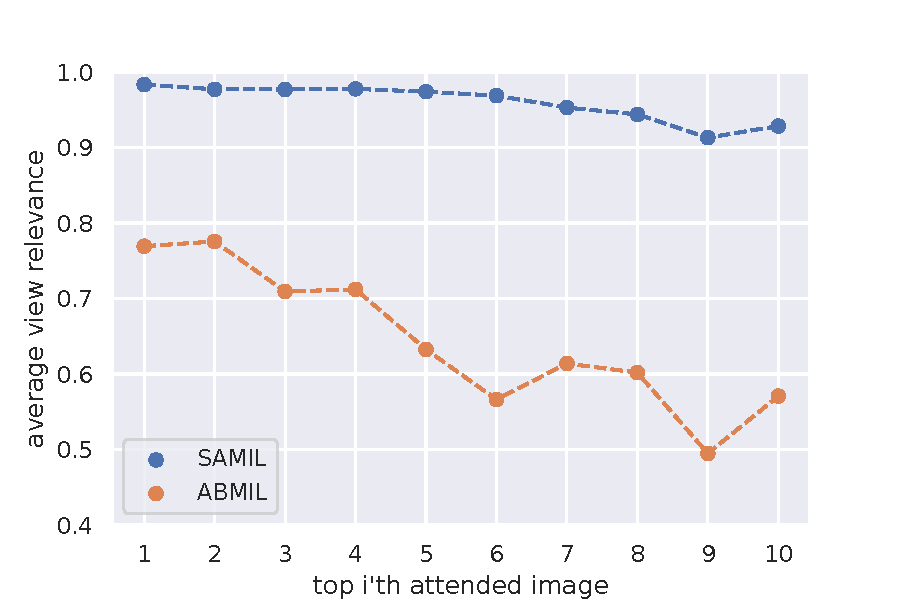
\includegraphics[width=0.32\textwidth]{figures/Attention_View_Alignment/data_seed2.pdf}
    \end{tabular}	
    \caption{
    Predicted view relevance of top-ranked images by attention (higher is better).
    %Showing the attention weights and view relevance alignment across all studies in the test set for multiple train/test splits. 
    Supervised attention (SAMIL, ours) outperforms off-the-shelf ABMIL by wide margin across all 3 splits.
    The x-axis indicates a rank position of images within an echo study when sorted by attention (1 = largest $a_k$, 2 = second largest, etc.). The y-axis indicates the average view relevance (across studies in test set) assigned by view classifier $v(x)$ to image $x$ at rank $k$. 
     }
    \label{fig:Attention_View_Alignment}
\end{figure}